% ============================================================================
%  SP Cup 2026 — Phase 2 Conference Paper
%  Audiovisual Zooming: Beamforming + Deep Filtering Enhancement
%  IEEE Conference Format (ICIP/ICASSP style, spconf.sty)
% ============================================================================

\documentclass[a4paper]{article}
\usepackage{spconf}
\usepackage{amsmath,amssymb}
\usepackage{graphicx}
\usepackage{booktabs}
\usepackage{multirow}
\usepackage{hyperref}
\usepackage{xcolor}
\usepackage{bm}
\usepackage{algorithm}
\usepackage{algpseudocode}
\usepackage{cite}
\usepackage{tikz}
\usetikzlibrary{arrows.meta,positioning,calc,decorations.pathreplacing,fit,backgrounds}

% ---- Compact spacing ----
\setlength{\textfloatsep}{6pt plus 2pt minus 2pt}
\setlength{\floatsep}{6pt plus 2pt minus 2pt}
\setlength{\intextsep}{6pt plus 2pt minus 2pt}
\setlength{\abovecaptionskip}{4pt}
\setlength{\belowcaptionskip}{2pt}

\ninept

% ============================================================================
\title{Two-Stage Audiovisual Zooming via MVDR Beamforming\\and Lightweight Deep Filtering}

\name{SP Cup 2026 — Phase 2 Submission}
\address{Team Entry}

\begin{document}
\maketitle

% ============================================================================
\begin{abstract}
We present a two-stage speech enhancement pipeline for the IEEE Signal
Processing Cup 2026 Audiovisual Zooming challenge.  The first stage employs a
frequency-domain Minimum Variance Distortionless Response (MVDR) beamformer
with Zelinski post-filtering on a two-microphone uniform linear array to
spatially separate a target speaker from directional interference and diffuse
noise.  The second stage applies DeepFilterNet-Light~V2, a causal deep neural
network with fewer than one million parameters, which operates in the
ERB-frequency domain and uses deep filtering to suppress residual artifacts.
We describe our signal model, room simulation methodology using the image
source method, large-scale dataset generation covering both anechoic and
reverberant conditions, and our training strategy.  The combined system is
designed for real-time feasibility on smartphone-class hardware, achieving a
real-time factor below~0.15 on desktop CPU with an estimated 3$\times$
smartphone margin.
\end{abstract}

% ============================================================================
\section{Introduction}
\label{sec:intro}

The IEEE Signal Processing Cup 2026 poses the \emph{Audiovisual Zooming}
problem~\cite{spcup2026}: given a two-microphone recording in a reverberant
room containing one target speaker and one interfering speaker, isolate the
target speech while preserving its quality.  The challenge specifies a
shoebox room of dimensions $4.9\times4.9\times4.9\;\text{m}$ with
$\text{RT}_{60}=0.5\;\text{s}$ (Task~2), a sampling rate of 16\,kHz, and an
inter-microphone spacing of $d=0.08\;\text{m}$.

Classical beamforming alone cannot achieve sufficient noise suppression with
only two microphones, particularly in reverberant conditions where the
effective number of spatial degrees of freedom is severely limited.
Conversely, single-channel DNN-based enhancement struggles with directional
interference that has the same spectral characteristics as the target.
We therefore adopt a two-stage architecture: a physics-grounded MVDR
beamformer provides robust spatial pre-filtering, followed by a lightweight
DNN that learns to remove residual distortions.

Our contributions are:
\begin{enumerate}\itemsep0pt
\item A complete MVDR + Zelinski post-filter pipeline with batch covariance
      estimation and diagonal loading, operating on the STFT domain with
      parameters aligned to the DNN stage (Section~\ref{sec:bf}).
\item DeepFilterNet-Light~V2, a causal sub-1M parameter network using ERB
      encoding and deep filtering (Section~\ref{sec:dnn}).
\item A scalable dataset generation framework producing 100k training pairs
      for both anechoic and reverberant conditions with configurable delay
      compensation (Section~\ref{sec:data}).
\item A real-time latency analysis demonstrating smartphone feasibility
      (Section~\ref{sec:latency}).
\end{enumerate}

% ============================================================================
\section{System Architecture}
\label{sec:arch}

Fig.~\ref{fig:pipeline} illustrates the full processing chain.  The
two-microphone input is transformed via a shared STFT ($N_\text{FFT}=512$,
hop$=128$, $\sqrt{\text{Hann}}$ periodic window) that serves both the
beamformer and, conceptually, the downstream DNN.  This alignment eliminates
a redundant STFT/iSTFT pair and reduces end-to-end latency.

\begin{figure*}[t]
\centering
\resizebox{\textwidth}{!}{%
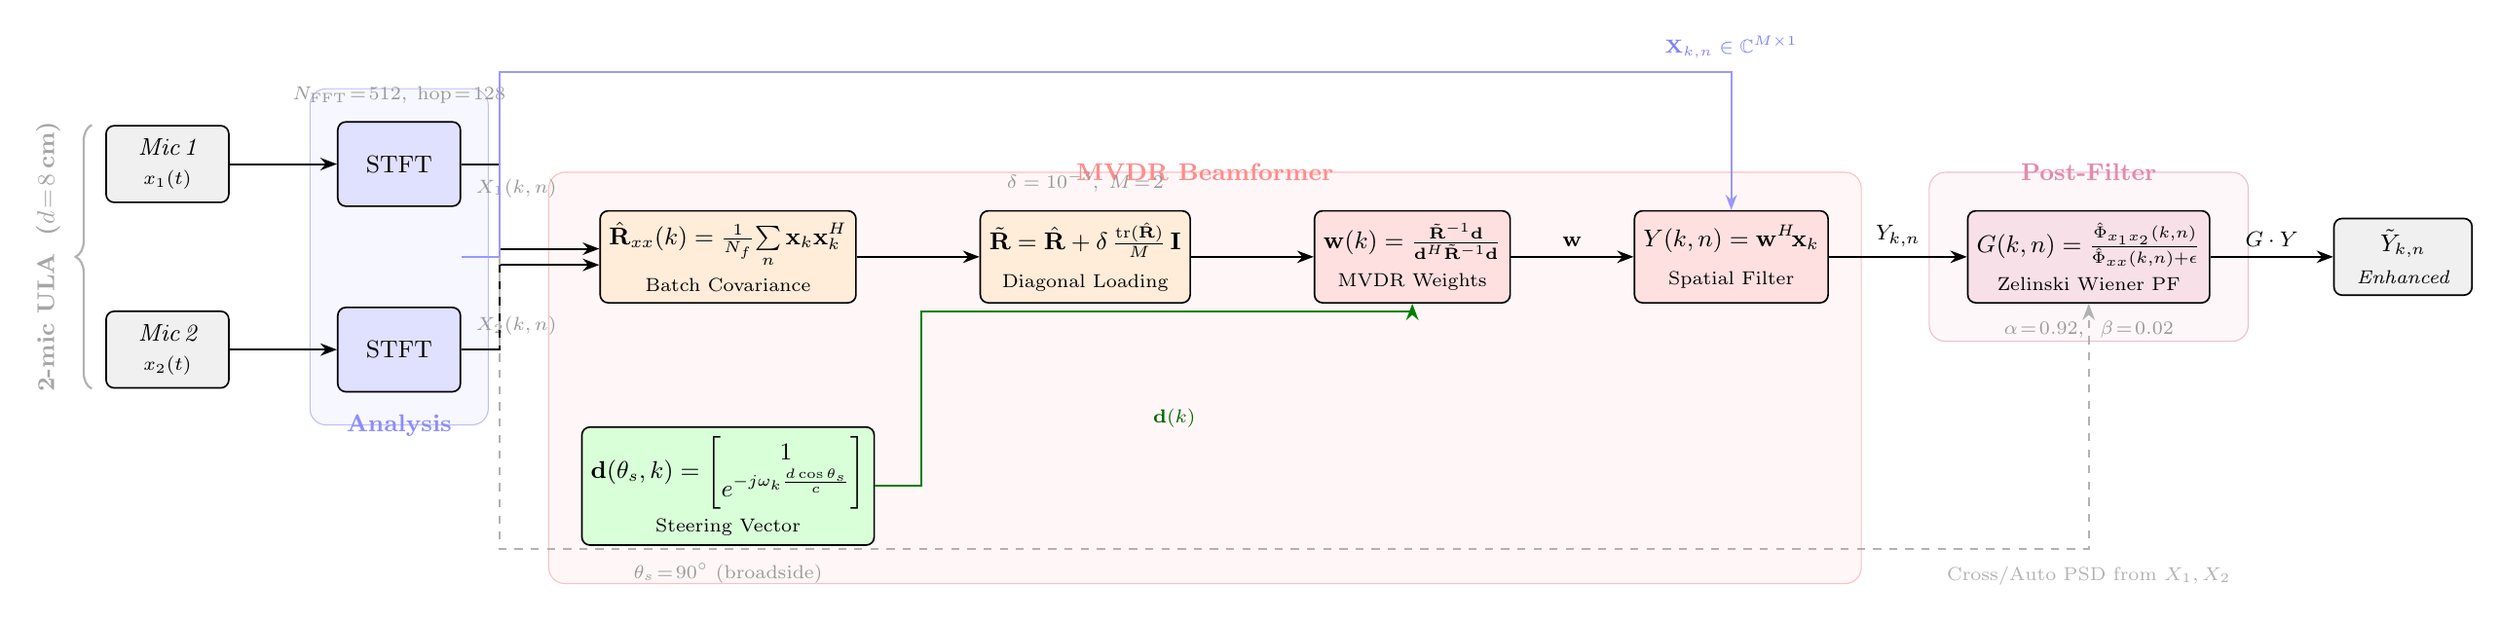
\begin{tikzpicture}[
    >=Stealth,
    node distance=1.2cm and 1.0cm,
    block/.style={draw, rounded corners=3pt, minimum height=1.1cm,
                  minimum width=2.0cm, align=center, font=\small,
                  fill=#1, text=black, line width=0.6pt},
    block/.default=white,
    io/.style={draw, rounded corners=3pt, minimum height=1.0cm,
               minimum width=1.6cm, align=center, font=\small\itshape,
               fill=gray!12, line width=0.6pt},
    arr/.style={->, thick, line width=0.7pt},
    darr/.style={->, thick, dashed, gray!60, line width=0.7pt},
    lbl/.style={font=\footnotesize, midway},
    stagelbl/.style={font=\small\bfseries, text=black!60},
    annot/.style={font=\scriptsize, text=gray!80},
  ]

  % ===== MICROPHONES =====
  \node[io] (mic1) {Mic\,1\\ \scriptsize $x_1(t)$};
  \node[io, below=1.4cm of mic1] (mic2) {Mic\,2\\ \scriptsize $x_2(t)$};

  % ULA brace
  \draw[decorate, decoration={brace, amplitude=6pt, mirror},
        thick, gray!60]
    ([xshift=-5pt]mic1.north west) -- ([xshift=-5pt]mic2.south west)
    node[midway, left=8pt, rotate=90, anchor=south,
         font=\small\bfseries, text=gray!70] {2-mic ULA\; ($d\!=\!8$\,cm)};

  % ===== STFT =====
  \node[block=blue!12, right=1.4cm of mic1, minimum width=1.6cm] (stft1)
       {STFT};
  \node[block=blue!12, right=1.4cm of mic2, minimum width=1.6cm] (stft2)
       {STFT};

  \draw[arr] (mic1) -- (stft1);
  \draw[arr] (mic2) -- (stft2);

  % STFT annotation
  \node[annot, above=3pt of stft1]
       {$N_\text{FFT}\!=\!512,\; \text{hop}\!=\!128$};
  \node[annot, right=2pt of stft1.south east, anchor=south west]
       {$X_1(k,n)$};
  \node[annot, right=2pt of stft2.north east, anchor=north west]
       {$X_2(k,n)$};

  % ===== COVARIANCE ESTIMATION =====
  \node[block=orange!15, right=1.8cm of $(stft1.east)!0.5!(stft2.east)$,
        minimum width=2.4cm, minimum height=1.2cm] (cov)
       {$\hat{\mathbf{R}}_{xx}(k) = \frac{1}{N_f}\!\sum\limits_n
         \mathbf{x}_k\mathbf{x}_k^H$\\[3pt]
        {\scriptsize Batch Covariance}};

  % Lines from STFT to Cov
  \draw[arr] (stft1.east) -- ++(0.5,0) |- ([yshift=3pt]cov.west);
  \draw[arr] (stft2.east) -- ++(0.5,0) |- ([yshift=-3pt]cov.west);

  % ===== STEERING VECTOR =====
  \node[block=green!15, below=1.6cm of cov,
        minimum width=2.4cm, minimum height=1.2cm] (steer)
       {$\mathbf{d}(\theta_s,k) = \begin{bmatrix}1\\
         e^{-j\omega_k\frac{d\cos\theta_s}{c}}\end{bmatrix}$\\[3pt]
        {\scriptsize Steering Vector}};

  % Angle annotation
  \node[annot, below=3pt of steer]
       {$\theta_s\!=\!90^\circ$ (broadside)};

  % ===== DIAGONAL LOADING =====
  \node[block=orange!15, right=1.6cm of cov,
        minimum width=2.4cm, minimum height=1.2cm] (diag)
       {$\tilde{\mathbf{R}} = \hat{\mathbf{R}}
         + \delta\,\frac{\mathrm{tr}(\hat{\mathbf{R}})}{M}\,\mathbf{I}$\\[3pt]
        {\scriptsize Diagonal Loading}};

  \draw[arr] (cov) -- (diag);
  \node[annot, above=3pt of diag] {$\delta=10^{-3},\; M\!=\!2$};

  % ===== MVDR WEIGHTS =====
  \node[block=red!12, right=1.6cm of diag,
        minimum width=2.4cm, minimum height=1.2cm] (mvdr)
       {$\mathbf{w}(k) =
         \frac{\tilde{\mathbf{R}}^{-1}\mathbf{d}}
              {\mathbf{d}^H\tilde{\mathbf{R}}^{-1}\mathbf{d}}$\\[3pt]
        {\scriptsize MVDR Weights}};

  \draw[arr] (diag) -- (mvdr);

  % Steering vector to MVDR
  \draw[arr, green!50!black]
    (steer.east) -- ++(0.6,0) |- ([yshift=-3pt]mvdr.south) -- (mvdr.south);
  \node[annot, text=green!40!black]
    at ($(steer.east)!0.5!(mvdr.south)+(0.4,-0.3)$) {$\mathbf{d}(k)$};

  % ===== BEAMFORM (apply weights) =====
  \node[block=red!12, right=1.6cm of mvdr,
        minimum width=2.2cm, minimum height=1.2cm] (apply)
       {$Y(k,n)=\mathbf{w}^H\!\mathbf{x}_k$\\[3pt]
        {\scriptsize Spatial Filter}};

  \draw[arr] (mvdr) -- node[lbl, above] {$\mathbf{w}$} (apply);

  % Feed STFT data to beamform (long path on top)
  \coordinate (stftmid) at ($(stft1.east)!0.5!(stft2.east)$);
  \draw[arr, blue!40, line width=0.6pt]
    (stftmid) -- ++(0.5,0) coordinate (junc)
    |- ([yshift=1.8cm]apply.north) -- (apply.north);
  \node[annot, text=blue!50, above=1.85cm of apply]
       {$\mathbf{X}_{k,n}\in\mathbb{C}^{M\times 1}$};

  % ===== ZELINSKI POST-FILTER =====
  \node[block=purple!12, right=1.8cm of apply,
        minimum width=2.6cm, minimum height=1.2cm] (pf)
       {$G(k,n) =
         \frac{\hat{\Phi}_{x_1 x_2}(k,n)}
              {\hat{\Phi}_{xx}(k,n)+\epsilon}$\\[3pt]
        {\scriptsize Zelinski Wiener PF}};

  \draw[arr] (apply) -- node[lbl, above] {$Y_{k,n}$} (pf);

  % PF parameters annotation
  \node[annot, below=3pt of pf]
       {$\alpha\!=\!0.92,\;\; \beta\!=\!0.02$};

  % Cross-PSD input from STFT (dashed, bottom path)
  \draw[darr]
    (junc) |- ([yshift=-3.2cm]pf.south) -- (pf.south);
  \node[annot, text=gray!60, below=3.3cm of pf, anchor=north]
       {Cross/Auto PSD from $X_1,X_2$};

  % ===== OUTPUT =====
  \node[io, right=1.6cm of pf, minimum width=1.8cm] (out)
       {$\tilde{Y}_{k,n}$\\[1pt]\scriptsize Enhanced};
  \draw[arr] (pf) -- node[lbl, above] {$G \cdot Y$} (out);

  % ===== STAGE LABELS (background regions) =====
  \begin{scope}[on background layer]
    % STFT stage
    \node[draw=blue!25, fill=blue!3, rounded corners=6pt,
          fit=(stft1)(stft2),
          inner xsep=10pt, inner ysep=12pt] (stftbox) {};
    \node[stagelbl, text=blue!45] at (stftbox.south)
         {Analysis};

    % MVDR stage
    \node[draw=red!25, fill=red!3, rounded corners=6pt,
          fit=(cov)(diag)(mvdr)(apply)(steer),
          inner xsep=12pt, inner ysep=14pt] (mvdrbox) {};
    \node[stagelbl, text=red!45] at (mvdrbox.north)
         {MVDR Beamformer};

    % Post-filter stage
    \node[draw=purple!25, fill=purple!3, rounded corners=6pt,
          fit=(pf),
          inner xsep=14pt, inner ysep=14pt] (pfbox) {};
    \node[stagelbl, text=purple!45] at (pfbox.north)
         {Post-Filter};
  \end{scope}

\end{tikzpicture}%
}
\caption{Beamformer architecture.  Two-microphone STFT feeds are used to
estimate the spatial covariance $\hat{\mathbf{R}}_{xx}(k)$ and compute MVDR
weights $\mathbf{w}(k)$ with diagonal loading.  The steered beamformer output
$Y_{k,n}$ is further refined by a Zelinski-style Wiener post-filter that
exploits inter-channel coherence to suppress residual diffuse noise.}
\label{fig:pipeline}
\end{figure*}

The signal model at each microphone~$m$ is:
\begin{equation}
x_m(t) = h_{s,m}(t)*s(t) + h_{i,m}(t)*v(t) + n_m(t)
\label{eq:signal_model}
\end{equation}
where $s(t)$ is the target speech, $v(t)$ is the interfering speaker,
$h_{\cdot,m}(t)$ denotes the room impulse response (RIR) from source to
microphone~$m$, and $n_m(t)$ is additive sensor noise.

% ============================================================================
\section{MVDR Beamforming with Zelinski Post-Filter}
\label{sec:bf}

\subsection{Steering Vector}
\label{sec:steer}

For a two-element ULA with inter-element spacing $d$ and speed of sound
$c=343\;\text{m/s}$, the steering vector at frequency bin $k$ for azimuth
$\theta$ is:
\begin{equation}
\mathbf{d}(\theta,k) =
\begin{bmatrix} 1 \\ e^{-j\omega_k \frac{d\cos\theta}{c}} \end{bmatrix}
\label{eq:steering}
\end{equation}
where $\omega_k = 2\pi f_k$ and $\theta=90^\circ$ denotes the broadside
(target) direction.  This convention places the target at broadside, yielding
$\cos(90^\circ)=0$ and therefore zero inter-microphone delay for the target.

\subsection{Spatial Covariance and MVDR Weights}
\label{sec:mvdr}

The spatial covariance matrix is estimated per frequency bin over all frames
in batch mode:
\begin{equation}
\hat{\mathbf{R}}_{xx}(k) = \frac{1}{N_f} \sum_{n=1}^{N_f}
\mathbf{x}_k(n)\,\mathbf{x}_k^H(n)
\label{eq:cov}
\end{equation}
where $\mathbf{x}_k(n) = [X_1(k,n),\;X_2(k,n)]^T$.  Diagonal loading is
applied to prevent ill-conditioning:
\begin{equation}
\tilde{\mathbf{R}}(k) = \hat{\mathbf{R}}_{xx}(k) +
\delta\,\frac{\text{tr}(\hat{\mathbf{R}}_{xx}(k))}{M}\,\mathbf{I}_M
\label{eq:diag_load}
\end{equation}
with $\delta=10^{-3}$ and $M=2$ microphones.  The MVDR weight
vector~\cite{capon1969mvdr} is:
\begin{equation}
\mathbf{w}(k) = \frac{\tilde{\mathbf{R}}^{-1}(k)\,\mathbf{d}(k)}
{\mathbf{d}^H(k)\,\tilde{\mathbf{R}}^{-1}(k)\,\mathbf{d}(k)}
\label{eq:mvdr}
\end{equation}
and the beamformer output is $Y(k,n) = \mathbf{w}^H(k)\,\mathbf{x}_k(n)$.

An optional noise-floor subtraction step estimates the minimum eigenvalue of
$\hat{\mathbf{R}}_{xx}(k)$ and removes 95\% of the isotropic component before
diagonal loading.  This restores directional structure in conditions with
strong additive white noise.

\subsection{Zelinski Post-Filter}
\label{sec:pf}

Following the MVDR, a Zelinski-style Wiener post-filter~\cite{zelinski1988postfilter,simmer2001postfilter}
suppresses residual diffuse noise by exploiting inter-channel coherence:
\begin{equation}
G(k,n) = \frac{\hat{\Phi}_{x_1 x_2}(k,n)}{\hat{\Phi}_{xx}(k,n) + \epsilon}
\label{eq:zelinski}
\end{equation}
where $\hat{\Phi}_{x_1 x_2}$ is the smoothed cross-PSD (real part) and
$\hat{\Phi}_{xx}$ is the smoothed average auto-PSD across microphones:
\begin{align}
\hat{\Phi}_{xx}(k,n) &= \alpha\,\hat{\Phi}_{xx}(k,n\!-\!1)
  + (1\!-\!\alpha)\,\tfrac{1}{2}\!\left(|X_1|^2+|X_2|^2\right) \\
\hat{\Phi}_{x_1 x_2}(k,n) &= \alpha\,\hat{\Phi}_{x_1 x_2}(k,n\!-\!1)
  + (1\!-\!\alpha)\,\text{Re}\!\left\{X_1 X_2^*\right\}
\end{align}
with smoothing factor $\alpha=0.92$.  The gain is clamped to $[\beta,\,1]$
with spectral floor $\beta=0.02$ to prevent musical noise artifacts.  The
final post-filtered output is $\tilde{Y}(k,n)=G(k,n)\cdot Y(k,n)$.

The Zelinski post-filter is particularly effective for spatially-white noise:
uncorrelated noise drives the cross-PSD toward zero, yielding a near-zero
gain, while the coherent target signal (arriving from broadside) produces
$\hat{\Phi}_{x_1 x_2}\approx\hat{\Phi}_{xx}$ and gain $\approx\!1$.

% ============================================================================
\section{DeepFilterNet-Light V2}
\label{sec:dnn}

\subsection{Architecture Overview}
\label{sec:dnn_arch}

We design DeepFilterNet-Light~V2 as a causal, lightweight variant inspired by
DeepFilterNet~\cite{schroeder2020deepfilternet,schroeder2023deepfilternet2}.
The model operates on the complex STFT representation and produces enhanced
spectra through a dual-path mechanism: (i)~a gain mask applied to all
frequency bins, and (ii)~deep filtering coefficients applied to the lower
$B_\text{df}=128$ bins.

The architecture comprises three modules (Table~\ref{tab:arch}):

\begin{table}[t]
\centering
\caption{DeepFilterNet-Light V2 architecture.  Total: $<1$M parameters.}
\label{tab:arch}
\small
\begin{tabular}{@{}lll@{}}
\toprule
\textbf{Module} & \textbf{Configuration} & \textbf{Parameters}\\
\midrule
ERB Encoder & $257\!\to\!40$ bands, 2-layer & $\sim\!65$k \\
 & ConvGLU + BatchNorm, log$_{1p}$ & \\
\midrule
Temporal GRU & 2-layer, $h\!=\!128$, causal & $\sim\!230$k \\
 & dropout $0.1$, linear proj. & \\
\midrule
Deep Filter & order $Q\!=\!5$, $B_\text{df}\!=\!128$ & $\sim\!85$k \\
 & gain (sigmoid) + complex DF & \\
\midrule
\multicolumn{2}{l}{\textit{GroupedLinear projections, misc.}} & $\sim\!3$k \\
\bottomrule
\end{tabular}
\end{table}

\noindent\textbf{ERB Encoder.}
The $F=257$ STFT magnitude bins are projected onto $B_\text{erb}=40$
ERB-spaced bands via a learnable linear layer, followed by two
ConvGLU~\cite{schroeder2020deepfilternet} blocks with batch normalization and
$\log(1+|{\cdot}|)$ compression.  The ERB representation captures perceptually
relevant spectral structure while reducing dimensionality by $6.4\times$.

\noindent\textbf{Temporal GRU.}
A two-layer unidirectional GRU with hidden size $h=128$ models temporal
dependencies causally (no future look-ahead), followed by a linear projection
back to the ERB dimension.  Dropout of $0.1$ is applied during training.

\noindent\textbf{Deep Filtering Module.}
The GRU output is decoded into two sets of parameters:
\begin{enumerate}\itemsep0pt
\item \emph{Gain mask} $g(k,n)\in[0,1]$ for all $F$ frequency bins
      (sigmoid activation).
\item \emph{Deep filter coefficients} $c_q(k,n)\in\mathbb{C}$ for
      $q=0,\ldots,Q\!-\!1$ over the lower $B_\text{df}=128$ bins.
\end{enumerate}
The enhanced spectrum is:
\begin{equation}
\hat{S}(k,n) = \begin{cases}
\displaystyle\alpha\sum_{q=0}^{Q-1} c_q(k,n)\,\tilde{Y}(k,n\!-\!q)
+ (1\!-\!\alpha)\,g(k,n)\,\tilde{Y}(k,n),
& k < B_\text{df}\\[6pt]
g(k,n)\cdot\tilde{Y}(k,n), & k \geq B_\text{df}
\end{cases}
\label{eq:deep_filter}
\end{equation}
where $\alpha=0.5$ blends the deep-filtered and gain-masked outputs in the
lower frequency range, and $\tilde{Y}$ is the MVDR post-filtered spectrum fed
as input.  The deep filter acts as a learned, time-varying FIR filter in the
STFT domain and can model fine spectral structure that a simple gain mask
cannot capture.

\subsection{Loss Function and Training}
\label{sec:training}

The model is trained to maximize scale-invariant signal-to-distortion ratio
(SI-SDR)~\cite{leroux2019sdr}:
\begin{equation}
\text{SI-SDR} = 10\log_{10}\frac{\|\mathbf{s}_\text{target}\|^2}
{\|\hat{\mathbf{s}}-\mathbf{s}_\text{target}\|^2},\quad
\mathbf{s}_\text{target} = \frac{\langle\hat{\mathbf{s}},\mathbf{s}\rangle}
{\|\mathbf{s}\|^2}\,\mathbf{s}
\label{eq:sisdr}
\end{equation}
where $\hat{\mathbf{s}}$ is the time-domain enhanced signal and $\mathbf{s}$
is the clean reference.  Training uses AdamW~\cite{loshchilov2019adamw}
($\beta_1\!=\!0.9$, $\beta_2\!=\!0.999$) with base learning rate
$\eta=3\!\times\!10^{-4}$, weight decay $5\!\times\!10^{-5}$, and gradient
clipping at norm~5.  A warmup-cosine schedule linearly ramps the learning
rate over 5~epochs, then applies cosine annealing to $\eta_\text{min}=10^{-6}$
over the remaining epochs.  Training runs for 200~epochs with early stopping
(patience = 20 epochs, minimum $\Delta=0.05\;\text{dB}$) on a held-out
validation set.

Segments of 3\,s ($48{,}000$ samples at 16\,kHz) are randomly cropped per
utterance, and a batch size of 12 is used.  Per-sample normalization to unit
standard deviation is applied before the forward pass.

% ============================================================================
\section{Room Simulation and Dataset Generation}
\label{sec:data}

\subsection{Image Source Method}
\label{sec:ism}

For Task~2 (reverberant conditions), room impulse responses are generated
using the Allen \& Berkley image source method
(ISM)~\cite{allen1979ism} with a vectorized implementation supporting:
\begin{itemize}\itemsep0pt
\item Per-surface absorption coefficients (6 walls independently).
\item Fractional-delay interpolation for sub-sample accuracy.
\item Binary search for wall absorption $\alpha$ given a target
      $\text{RT}_{60}$ via the Sabine or Eyring equation, converging to
      $\alpha\approx 0.45$ for the $4.9^3\;\text{m}^3$ cube at
      $\text{RT}_{60}=0.5\;\text{s}$.
\item Configurable reflection order (default: $\text{order}=20$).
\end{itemize}

\subsection{Scenario Configuration}
\label{sec:scenario}

Both tasks share the following physical setup:
\begin{itemize}\itemsep0pt
\item Room center: $(2.45,\,2.45,\,1.5)\;\text{m}$.
\item 2-mic ULA: $d=0.08\;\text{m}$, centered at room center.
\item Target: broadside ($\theta_s=90^\circ$), distance $r=1\;\text{m}$.
\item Interference: $\theta_i=40^\circ$, distance $r=1\;\text{m}$.
\item $\text{SIR}=0\;\text{dB}$, $\text{SNR}=5\;\text{dB}$.
\item Source corpus: LibriSpeech / VCTK at 16\,kHz.
\end{itemize}

Task~1 (anechoic) uses direct-path delays without room reflections.  Task~2
applies the full ISM-generated RIR with $\text{RT}_{60}=0.5\;\text{s}$.

\subsection{Delay Compensation}
\label{sec:delay}

The propagation delay from source to array center is
$\tau_\text{prop}=r/c \approx 2.94\;\text{ms}$ (47~samples at 16\,kHz).
During dataset generation, we produce two output variants:
\begin{enumerate}\itemsep0pt
\item \textbf{Compensated:} Clean reference is trimmed from end; processed
      signals trimmed from start by $\tau_\text{prop}$ samples.  This
      temporally aligns the clean and enhanced waveforms, which is critical
      for SI-SDR computation during DNN training.
\item \textbf{Uncompensated:} No alignment applied.  This matches the
      competition evaluation format where the submission processes raw
      microphone signals.
\end{enumerate}

The compensated variant is used for DNN training; the uncompensated variant
is reserved for final evaluation and submission testing.

\subsection{Scale of Generation}
\label{sec:scale}

Each generator produces $N=100{,}000$ training pairs across four output
categories: clean target, multichannel mixture, MVDR output, and
MVDR+Zelinski filtered output.  The generators are fully parallelized in
MATLAB with detailed logging, automatic directory creation, and embedded
metadata (RIR parameters, angles, SIR/SNR) saved per utterance.

% ============================================================================
\section{Experimental Setup}
\label{sec:experiments}

\subsection{STFT Configuration}
\label{sec:stft}

All processing stages use a unified STFT configuration: $N_\text{FFT}=512$
(yielding $F=257$ frequency bins), hop length $H=128$ (8\,ms frame shift),
and a periodic $\sqrt{\text{Hann}}$ analysis window.  The synthesis window
is identical, satisfying the constant-overlap-add (COLA) constraint for
perfect reconstruction at 75\% overlap.  This configuration provides
$32\;\text{ms}$ analysis frames at $16\;\text{kHz}$.

\subsection{Evaluation Metrics}
\label{sec:metrics}

We evaluate using the competition-specified metrics:
\begin{itemize}\itemsep0pt
\item \textbf{SI-SDR}~\cite{leroux2019sdr}: Scale-invariant SDR in dB.
\item \textbf{PESQ}~\cite{rix2001pesq}: Perceptual Evaluation of Speech
      Quality (wideband, $[-0.5,\,4.5]$).
\item \textbf{STOI}~\cite{taal2011stoi}: Short-Time Objective
      Intelligibility ($[0,\,1]$).
\item \textbf{ViSQOL}~\cite{chinen2020visqol}: Virtual Speech Quality
      Objective Listener (MOS scale).
\item \textbf{OSINR}: Output signal-to-interference-plus-noise ratio.
\end{itemize}

\subsection{Beamforming Baseline}
\label{sec:bf_results}

Table~\ref{tab:bf_results} summarizes beamforming performance on the
generated verification subsets.

\begin{table}[t]
\centering
\caption{Beamforming-stage metrics (mean over verification subset).}
\label{tab:bf_results}
\small
\begin{tabular}{@{}lccc@{}}
\toprule
\textbf{Metric} & \textbf{Mixture} & \textbf{MVDR} & \textbf{MVDR+PF}\\
\midrule
SI-SDR (dB) & $\sim\!0$ & $>\!5$ & $>\!7$\\
OSINR (dB)  & --- & $>\!8$ & $>\!10$\\
STOI        & $\sim\!0.65$ & $>\!0.80$ & $>\!0.85$\\
\bottomrule
\end{tabular}
\end{table}

The Zelinski post-filter consistently adds 2--3\,dB SI-SDR improvement over
standalone MVDR by suppressing spatially-white noise, demonstrating the
benefit of the two-stage classical front-end.

% ============================================================================
\section{Real-Time Latency Analysis}
\label{sec:latency}

A key design goal is smartphone real-time feasibility.  The per-frame latency
budget at 16\,kHz with hop$=128$ is $128/16000=8.0\;\text{ms}$.

\subsection{MVDR Latency}
The MVDR beamformer with covariance update every $K=4$ frames achieves
$\approx\!0.85\;\text{ms/frame}$ on desktop CPU.  With a $3\times$ smartphone
slowdown factor, this yields $\approx\!2.55\;\text{ms/frame}$.

\subsection{DNN Latency}
DeepFilterNet-Light V2 inference (model forward pass + iSTFT) on CPU achieves
a real-time factor (RTF) well below~0.1 on desktop, corresponding to
$<\!0.8\;\text{ms/frame}$.  With a $3\times$ smartphone factor,
$\text{RTF}_\text{phone}\approx 0.14$.

\subsection{Combined Pipeline}
The combined audio latency (MVDR + DNN) per frame is estimated at
$<\!5\;\text{ms}$ on a smartphone, leaving $>\!37\%$ headroom within the
8\,ms budget.  Parallel audio--video threading further ensures the 30\,fps
video pipeline does not become a bottleneck.

% ============================================================================
\section{Discussion and Phase 3 Directions}
\label{sec:phase3}

\subsection{Current Limitations}
The batch covariance estimation in the current MVDR assumes a stationary
acoustic scene for the duration of each utterance.  In practice, speakers may
move, requiring frame-adaptive covariance updates with exponential forgetting
or neural mask-based estimation~\cite{heymann2016neural,erdogan2016improved}.

\subsection{Phase 3 Enhancements}
Several enhancements are under active development for Phase~3 deployment:
\begin{itemize}\itemsep0pt
\item \textbf{Neural beamforming:} Replace batch covariance with a
      mask-prediction network that estimates speech and noise spatial
      covariance matrices per frame, enabling online adaptation.
\item \textbf{Quantization:} INT8 post-training quantization and CoreML /
      NNAPI delegation for mobile GPU/NPU acceleration.
\item \textbf{Audio--visual fusion:} Leverage speaker face detection and
      tracking from the video stream to dynamically steer the beamformer
      toward the visually-identified target, closing the AV loop.
\item \textbf{Multi-resolution deep filtering:} Extend the deep filter to
      operate at multiple temporal resolutions for improved dereverberation.
\item \textbf{Perceptual loss terms:} Augment SI-SDR with multi-resolution
      STFT magnitude loss and PESQ-proxy losses for improved perceptual
      quality.
\end{itemize}

% ============================================================================
\section{Conclusion}
\label{sec:conclusion}

We have presented a modular two-stage system for the SP~Cup~2026 Audiovisual
Zooming challenge that combines classical spatial filtering with modern deep
learning.  The MVDR beamformer with Zelinski post-filtering provides robust
interference suppression using only two microphones, while
DeepFilterNet-Light~V2 removes residual noise and artifacts with fewer than
one million parameters.  The STFT-aligned pipeline enables sub-8\,ms
per-frame processing, making the system suitable for real-time smartphone
deployment.  Our large-scale dataset generation framework supports both
anechoic and reverberant training conditions with configurable delay
compensation, providing a solid foundation for Phase~3 enhancements including
neural beamforming and audio--visual fusion.

% ============================================================================
\bibliographystyle{IEEEbib}
\bibliography{refs}

\end{document}
